\documentclass[12pt]{article}

\usepackage[left=25mm, right=25mm, top=25mm, bottom=25mm, headheight=25mm]{geometry}
\usepackage{graphicx} % Required for inserting images
\usepackage{subfig} % Poder colocar más de una imagen en una {Figura}
\usepackage[figurename=Imagen]{caption} % Cambiar la descripción de la Image 
\usepackage[utf8]{inputenc} % Idioma español
\usepackage[spanish]{babel} % Idioma español

% Para poder ajustar los colores en las referencias que se hagan
\usepackage{hyperref}
\hypersetup{
    colorlinks=true,
    linkcolor = black,
    citecolor = blue,
    urlcolor = blue
}

% Dar formato a las páginas y colocar el \rfoot{De forma que nos interese}
\usepackage{parskip}
\usepackage{lastpage}
\usepackage{xcolor}
\usepackage{fancyhdr}
\pagestyle{fancy}
\cfoot{}
\rfoot{Página \thepage\ de \pageref{LastPage}}
\rhead{}
\lhead{}
\renewcommand{\headrulewidth}{0pt}

% Parámetros que pueden cambiar ----------------------------------------------------------------------------
% Nombres
\newcommand{\Profesor}{Profesor: Edgar Tista García}
\newcommand{\Materia}{Asignatura: Estructura de Datos y Algoritmos II}
\newcommand{\Grupo}{Grupo:  5}
\newcommand{\NumeroPra}{No. de práctica:  11, 12 y 13}
\newcommand{\Nombre}{Integrante:  Martínez Trinidad Alexis ,Quetzalli Zarate Menes}
\newcommand{\NoLista}{No. de lista:     22, 32}
\newcommand{\Semestre}{Semestre: 2024-2}
\newcommand{\Fecha}{Fecha de entrega:  17 de mayo del 2024}
\newcommand{\Observaciones}{Observaciones:}
\newcommand{\Calificacion}{CALIFICACIÓN:}

\newcommand{\TituloP}{Laboratorios de computación salas A y B}
\newcommand{\Titulo}{\NumeroPra\\\TituloP}

\begin{document}    
    \begin{center}
        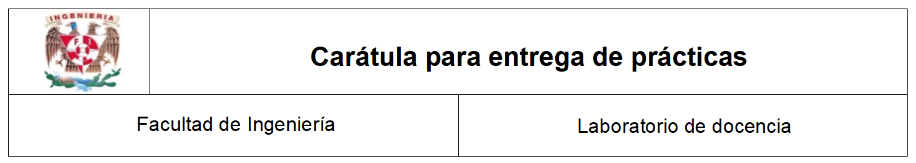
\includegraphics[width=\textwidth]{Images/titulo.png}
        \LARGE\textbf{\TituloP}\par\vspace{0.7cm}
    \end{center}
    \Large{\Profesor}\par\vspace{0.6cm}
    \Large{\Materia}\par\vspace{0.6cm}
    \Large{\Grupo}\par\vspace{0.6cm}
    \Large{\NumeroPra}\par\vspace{0.6cm}
    \Large{\Nombre}\par\vspace{0.6cm}
    \Large{\NoLista}\par\vspace{0.6cm}
    \Large{\Semestre}\par\vspace{0.6cm}
    \Large{\Fecha}\par\vspace{0.6cm}
    \Large{\Observaciones}\par\vspace{0.6cm}

    \begin{center}
        \Large{\Calificacion}\par\vspace{0.6cm}
    \end{center}
% -------------------------------------------------------- Empieza el desarrollo de la práctica
    
    \newpage
    \textcolor{blue}{\textbf{OBJETIVO}}
    PRACTICA #11: Introducción a OpenMP
    OBJETIVO: EL ESTUDIANTE CONOCERÁ Y APRENDERÁ A UTILIZAR ALGUNAS DE LAS DIRECTIVAS DE 
    OPENMP UTILIZADAS PARA REALIZAR PROGRAMAS PARALELOS.


    \par\vspace{1.5cm}

    \textcolor{blue}{\textbf{ANÁLISIS}}


    \textcolor[rgb]{0.13, 0.55, 0.13}{\textbf{c)}}




    \textcolor{blue}{\textbf{CONCLUSIONES}}
























    \end{document}